\documentclass{article}

%% doc settings
\hyphenchar\font=-1 % suppress hyphenation
\setlength\parindent{0pt} % suppress indentation
\usepackage[margin=1.5truein]{geometry} % set page margins

%% libraries
\usepackage{listings}
\usepackage{fancyhdr}
\usepackage{lastpage}
\usepackage{url}
\usepackage{xcolor}
\usepackage{hyperref}
\usepackage{natbib}
\usepackage{tikz}
\usepackage{pgfplots}
\usepackage{textcomp}
\usepackage{subcaption}
\usetikzlibrary{shapes, arrows}

%% link viz
\hypersetup{
    colorlinks = true,
    linkcolor = red,
    urlcolor = red,
    citecolor = black
}

%% page nums
\pagestyle{fancy}
\fancyhf{}
\fancyfoot[C]{Pg. \thepage \space of \pageref*{LastPage}}
\renewcommand{\headrulewidth}{0pt}

%% begin doc
\begin{document}
\title{SYSEN 6000: Foundations of Complex Systems\\~\\
    \Large Networks \& Matrices
}
\author{
    Nick Kunz [NetID: \url{nhk37}] \hyperlink{nhk37@cornell.edu}{nhk37@cornell.edu}}
\date{October 14, 2022}
\maketitle
\thispagestyle{fancy}

\section*{Washington I-5 Corridor Interstate Highway System}
This is a basic network analysis of the Washington I-5 corridor interstate highway system containing the following four parts: 1) Geographic Map, 2) Graph Network, 3) Adjacency Matrix, 4) Histogram of Connected Edges

\subsection*{Geographic Map}
The following is a geographic map of Washington State identifying 10 major population centers along the I-5 corridor (north-south), as well as the broader interstate highway system connecting them (bold lines).
    \begin{figure}[h]
        \centering
        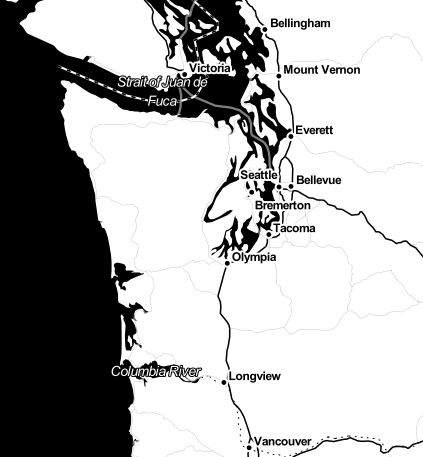
\includegraphics[width=0.55\textwidth]{pnw_map.png}
        \caption{Washington I-5 Corridor Geographic Map \cite{folium}}
        \label{fig:geomap}
    \end{figure}

\newpage
\subsection*{Graph Network}
The following is a graph network representing the interstate highway system in the geographic map (Figure \ref{fig:geomap}). All other road systems, such as state and local highways, were beyond the scope of this analysis and not included here.
    \begin{figure}[h]
    \centering
    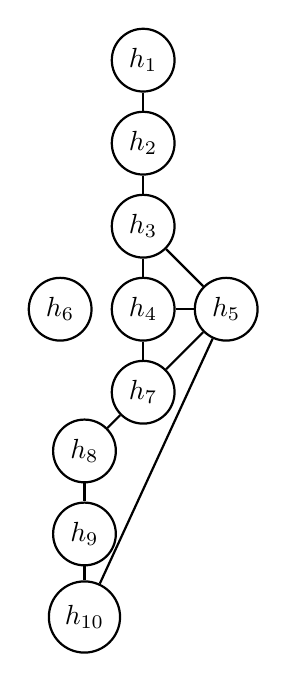
\begin{tikzpicture}[-,>=stealth',auto,node distance=30pt,
      thick,main node/.style={circle,,draw}, other node/.style={}]
    
        \node[main node] (1) {$h_1$};
        \node[main node] (2) [below of=1] {$h_2$};
        \node[main node] (3) [below of=2] {$h_3$};
        \node[main node] (4) [below of=3] {$h_4$};
        \node[main node] (5) [right of=4] {$h_5$};
        \node[main node] (6) [left of=4] {$h_6$};
        \node[main node] (7) [below of=4] {$h_7$};
        \node[main node] (8) [below left of=7] {$h_8$};
        \node[main node] (9) [below of=8] {$h_9$};
        \node[main node] (10) [below of=9] {$h_{10}$};
        
        \path[every node/.style={font=\sffamily\small}]
            (1) edge node [left] {} (2)
            (2) edge node [left] {} (3)
            (3) edge node [left] {} (4)
            (4) edge node [left] {} (5)
            (5) edge node [left] {} (3)
            (5) edge node [left] {} (7)
            (5) edge node [left] {} (10)
            (4) edge node [left] {} (7)
            (7) edge node [left] {} (8)
            (8) edge node [left] {} (9)
            (9) edge node [left] {} (10)
        ;
    \end{tikzpicture}
    \caption{Washington I-5 Corridor Graph Network}
    \label{fig:graph}
    \end{figure}

\subsection*{Adjacency Matrix}
The following is a matrix representation of the graph network (Figure \ref{fig:graph}). Notice that $h_6$ is included. However, not connected to the broader interstate system, and that $h_5$ and $h_{10}$ are connected, but not exhibited within the bounds of the geographic map (Figure \ref{fig:geomap}).

    \begin{figure}[h]
    \begin{equation} \nonumber
        A_h = \bordermatrix{
                 & h_1 & h_2 & h_3 & h_4 & h_5 & h_6 & h_7 & h_8 & h_9 & h_{10} \cr
             h_1 &   0   & 1   & 0   & 0   & 0   & 0   & 0   & 0   & 0   & 0    \cr
             h_2 &   1   & 0   & 1   & 0   & 0   & 0   & 0   & 0   & 0   & 0    \cr
             h_3 &   0   & 1   & 0   & 1   & 1   & 0   & 0   & 0   & 0   & 0    \cr
             h_4 &   0   & 0   & 1   & 0   & 1   & 0   & 1   & 0   & 0   & 0    \cr
             h_5 &   0   & 0   & 1   & 1   & 0   & 0   & 1   & 0   & 0   & 1    \cr
             h_6 &   0   & 0   & 0   & 0   & 0   & 0   & 0   & 0   & 0   & 0    \cr
             h_7 &   0   & 0   & 0   & 1   & 1   & 0   & 0   & 1   & 0   & 0    \cr
             h_8 &   0   & 0   & 0   & 0   & 0   & 0   & 1   & 0   & 1   & 0    \cr
             h_9 &   0   & 0   & 0   & 0   & 0   & 0   & 0   & 1   & 0   & 1    \cr
             h_{10} & 0   & 0   & 0   & 0   & 1   & 0   & 0   & 0   & 1   & 0   \cr
        }
    \end{equation}
    \caption{Washington I-5 Corridor Adjacency Matrix}
    \label{fig:matrix}
    \end{figure}
    
\newpage
where:
    \begin{center}
    \begin{tabular}{l}
        $h_1$ = Bellingham\\
        $h_2$ = Mount Vernon\\
        $h_3$ = Everett\\
        $h_4$ = Seattle\\
        $h_5$ = Bellevue\\
        $h_6$ = Bremerton\\
        $h_7$ = Tacoma\\
        $h_8$ = Olympia\\
        $h_9$ = Longview\\
        $h_{10}$ = Vancouver
    \end{tabular}
    \end{center}

\subsection*{Histogram of Connected Edges}
The following exhibit illustrates the ten major population centers ordered by the number of edges connecting them. Notice that $h_5$ (Bellevue) has the highest number of edges (four), and that $h_6$ (Bremerton) has the lowest number of edges (zero).

    \begin{figure}[h]
    \centering
    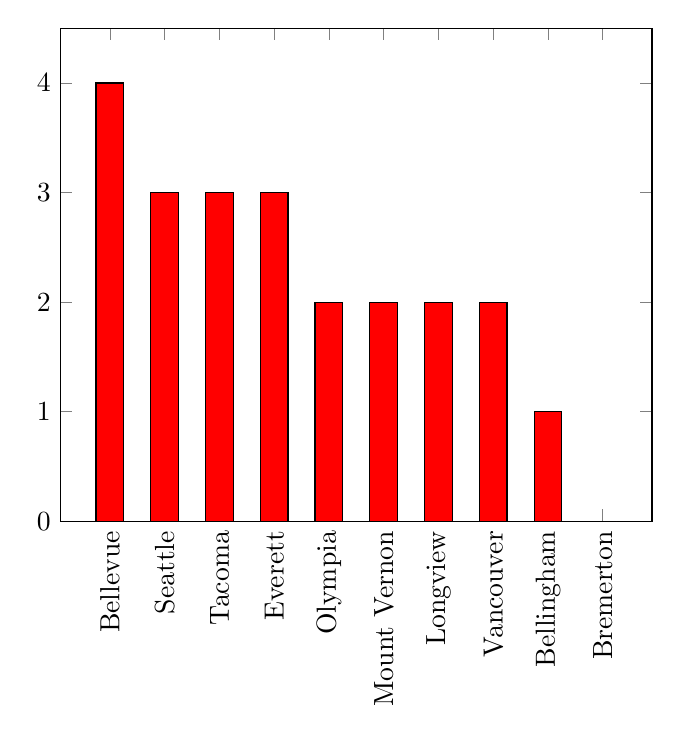
\begin{tikzpicture}
    \begin{axis}[
        width=\textwidth * 0.75,
        symbolic x coords={
            Bellevue,
            Seattle,
            Tacoma,
            Everett,
            Olympia,
            Mount Vernon,
            Longview,
            Vancouver,
            Bellingham,
            Bremerton
        },
        xtick=data,
        x tick label style={rotate=90,anchor=east},
        ymin=0, ymax=4.5, ytick={0,1,2,3,4}
        ]
        
        \addplot[ybar, fill=red] coordinates {
            (Bellevue, 4)
            (Seattle, 3)
            (Tacoma, 3)
            (Everett, 3)
            (Olympia, 2)
            (Mount Vernon, 2)
            (Longview, 2)
            (Vancouver, 2)
            (Bellingham, 1)
            (Bremerton, 0)
        };
    \end{axis}
    \end{tikzpicture}
    \caption{Washington I-5 Corridor Connected Edges}
    \label{fig:plot}
    \end{figure}
    
\section*{Japanese Shinkansen High Speed Rail System}
This is a basic network analysis of the Japanese Shinkansen high speed rail system containing the following four parts: 1) Geographic Map, 2) Graph Network, 3) Adjacency Matrix, 4) Histogram of Connected Edges

\subsection*{Geographic Map}
The following is a geographic map of the Japanese Shinkansen high speed rail system throughout broader Japan. This analysis is focused on only those cities which are northeast of Tokyo. 
    \begin{figure}[h]
        \centering
        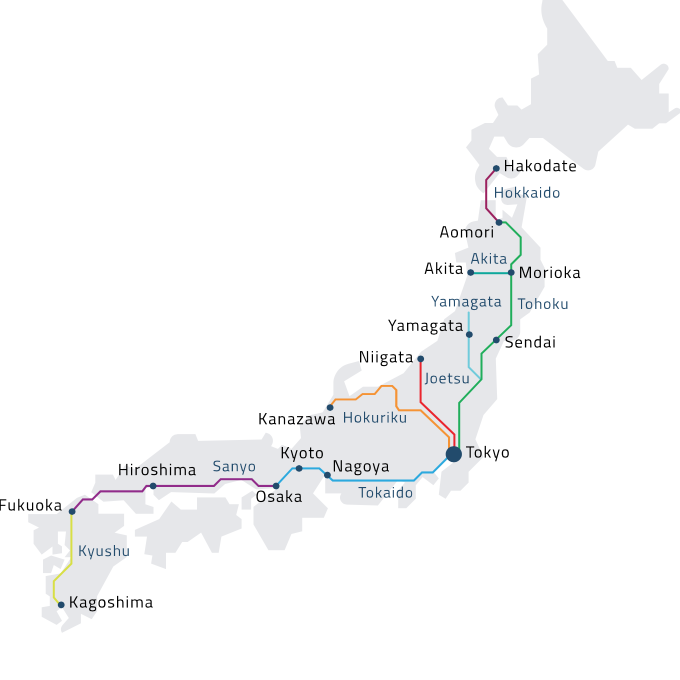
\includegraphics[width=0.67\textwidth]{jp_map.png}
        \caption{Japanese Shinkansen Geographic Map \cite{jrpass}}
        \label{fig:geomapjp}
    \end{figure}

\newpage
\subsection*{Graph Network}
The following is a graph network representing the high speed rail system northeast of Tokyo in the geographic map (Figure \ref{fig:geomapjp}). All other transportation systems, such as roads, were beyond the scope of this analysis and not included here.
    \begin{figure}[h]
    \centering
    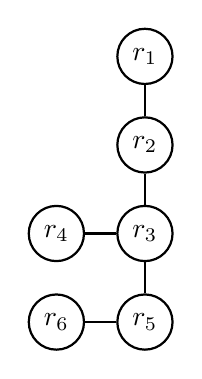
\begin{tikzpicture}[-,>=stealth',auto,node distance=32pt,
      thick,main node/.style={circle,,draw}, other node/.style={}]
    
        \node[main node] (1) {$r_1$};
        \node[main node] (2) [below of=1] {$r_2$};
        \node[main node] (3) [below of=2] {$r_3$};
        \node[main node] (4) [left of=3] {$r_4$};
        \node[main node] (5) [below of=3] {$r_5$};
        \node[main node] (6) [left of=5] {$r_6$};
        
        \path[every node/.style={font=\sffamily\small}]
            (1) edge node [left] {} (2)
            (2) edge node [left] {} (3)
            (3) edge node [left] {} (4)
            (3) edge node [left] {} (5)
            (5) edge node [left] {} (6)
        ;
    \end{tikzpicture}
    \caption{Japanese Shinkansen Graph Network (Northeast of Tokyo)}
    \label{fig:graphjp}
    \end{figure}

\subsection*{Adjacency Matrix}
The following is a matrix representation of the graph network (Figure \ref{fig:graphjp}). Notice that $r_5$ is the truncated node to the broader high speed rail system, and that $r_5$ is connected to Tokyo, but is not exhibited within the bounds of graph network (Figure \ref{fig:graphjp}).

    \begin{figure}[h]
    \begin{equation}
        A_r = \bordermatrix{
                 & r_1 & r_2 & r_3 & r_4 & r_5 & r_6 \cr
             r_1 &   0   & 1   & 0   & 0   & 0   & 0 \cr
             r_2 &   1   & 0   & 1   & 0   & 0   & 0 \cr
             r_3 &   0   & 1   & 0   & 1   & 1   & 0 \cr
             r_4 &   0   & 0   & 1   & 0   & 0   & 0 \cr
             r_5 &   0   & 0   & 1   & 0   & 0   & 1 \cr
             r_6 &   0   & 0   & 0   & 0   & 1   & 0 \cr
        }
    \end{equation}
    \caption{Japanese Shinkansen Adjacency Matrix (Northeast of Tokyo)}
    \label{fig:matrixjp}
    \end{figure}

    where:
    \begin{center}
    \begin{tabular}{l}
        $r_1$ = Hakodate\\
        $r_2$ = Aomori\\
        $r_3$ = Morioka\\
        $r_4$ = Akita\\
        $r_5$ = Sendai\\
        $r_6$ = Yamagata\\
    \end{tabular}
    \end{center}

\newpage
\subsection*{Histogram of Connected Edges}
The following exhibit illustrates the six major population centers ordered by the number of edges connecting them. Notice that $r_3$ (Morioka) has the highest number of edges (three), while $r_1$ (Hakodate), $r_2$ (Aomori), and $r_6$ (Yamagata) have the lowest number of edges (one).

    \begin{figure}[h]
    \centering
    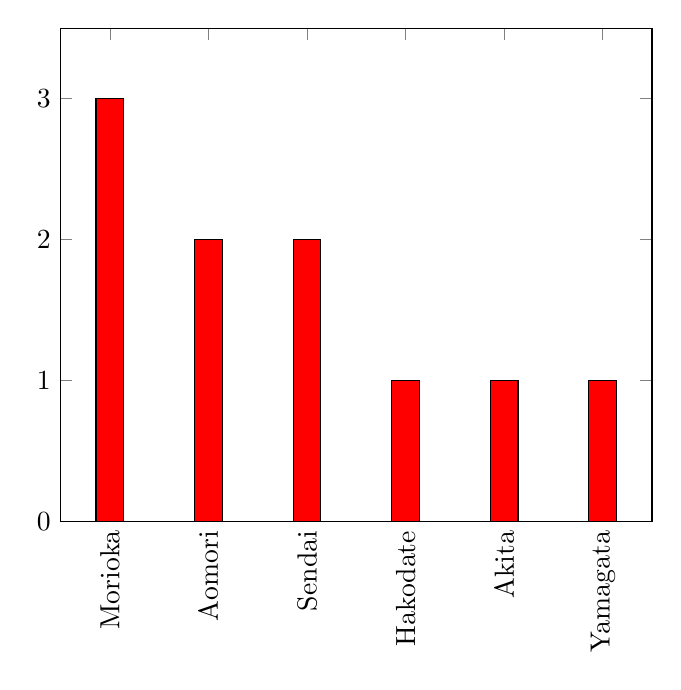
\begin{tikzpicture}
    \begin{axis}[
        width=\textwidth * 0.75,
        symbolic x coords={
            Morioka,
            Aomori,
            Sendai,
            Hakodate,
            Akita,
            Yamagata
        },
        xtick=data,
        x tick label style={rotate=90,anchor=east},
        ymin=0, ymax=3.5, ytick={0,1,2,3}
        ]
        
        \addplot[ybar, fill=red] coordinates {
            (Morioka, 3)
            (Aomori, 2)
            (Sendai, 2)
            (Hakodate, 1)
            (Akita, 1)
            (Yamagata, 1)
        };
    \end{axis}
    \end{tikzpicture}
    \caption{Japanese Shinkansen Connected Edges (Northeast of Tokyo)}
    \label{fig:plotjp}
    \end{figure}

\newpage
\section*{German Intercity-Express High Speed Rail System}
This is a basic network analysis of the German Intercity-Express (ICE) high speed rail system containing the following four parts: 1) Geographic Map, 2) Graph Network, 3) Adjacency Matrix, 4) Histogram of Connected Edges

\subsection*{Geographic Map}
The following is a geographic map of the German Intercity-Express high speed rail system throughout broader Germany. This analysis is focused on only those cities in the east south-east portion of the country.

    \begin{figure}[h]
        \centering
        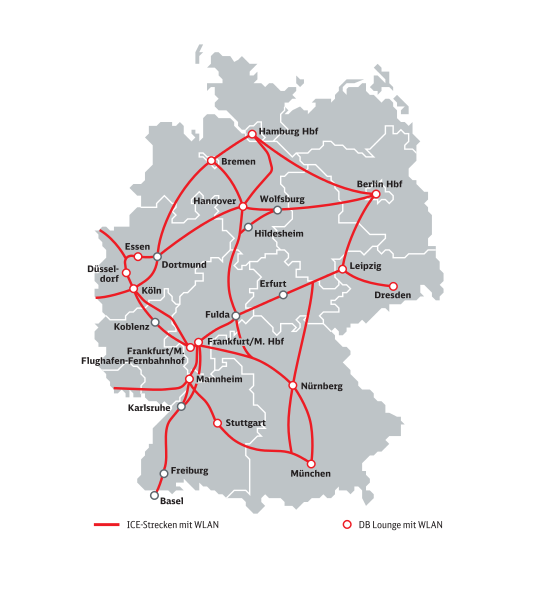
\includegraphics[width=0.75\textwidth]{ger_map.png}
        \caption{Germany Intercity-Express Geographic Map \cite{bahn}}
        \label{fig:geomapger}
    \end{figure}

\newpage
\subsection*{Graph Network}
The following is a graph network representing the high speed rail system in the east south-east portion of the geographic map (Figure \ref{fig:geomapger}). All other transportation systems, such as roads, were beyond the scope of this analysis and not included here.

    \begin{figure}[h]
    \centering
    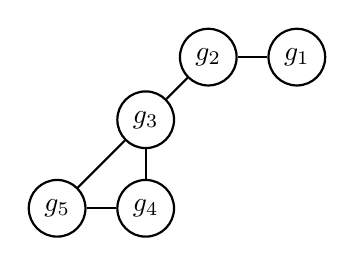
\begin{tikzpicture}[-,>=stealth',auto,node distance=32pt,
      thick,main node/.style={circle,,draw}, other node/.style={}]
    
        \node[main node] (1) {$g_1$};
        \node[main node] (2) [left of=1] {$g_2$};
        \node[main node] (3) [below left of=2] {$g_3$};
        \node[main node] (4) [below of=3] {$g_4$};
        \node[main node] (5) [left of=4] {$g_5$};
        
        \path[every node/.style={font=\sffamily\small}]
            (1) edge node [left] {} (2)
            (2) edge node [left] {} (3)
            (3) edge node [left] {} (4)
            (3) edge node [left] {} (5)
            (4) edge node [left] {} (5)
        ;
    \end{tikzpicture}
    \caption{Germany Intercity-Express Graph Network (East South-East Cities)}
    \label{fig:graphger}
    \end{figure}


\subsection*{Adjacency Matrix}
The following is a matrix representation of the graph network (Figure \ref{fig:graphger}). Notice that $g_2$, $g_3$, and $g_5$ are truncated nodes connected to the broader high speed rail system, but are not exhibited within the bounds of graph network (Figure \ref{fig:graphger).

    \begin{figure}[h]
    \begin{equation}
        A_g = \bordermatrix{
                 & g_1 & g_2 & g_3 & g_4 & g_5 \cr
             g_1 &   0   & 1   & 0   & 0   & 0 \cr
             g_2 &   1   & 0   & 1   & 0   & 0 \cr
             g_3 &   0   & 1   & 0   & 1   & 1 \cr
             g_4 &   0   & 0   & 1   & 0   & 1 \cr
             g_5 &   0   & 0   & 1   & 1   & 0 \cr
        }
    \end{equation}
    \caption{Germany Intercity-Express Adjacency Matrix (East South-East Cities)}
    \label{fig:matrixger}
    \end{figure}

    where:
    \begin{center}
    \begin{tabular}{l}
        $g_1$ = Dresden\\
        $g_2$ = Leipzig\\
        $g_3$ = Nurnberg\\
        $g_4$ = Munchen\\
        $g_5$ = Stuttgart\\
    \end{tabular}
    \end{center}

\newpage
\subsection*{Histogram of Connected Edges}
The following exhibit illustrates the five major population centers ordered by the number of edges connecting them. Notice that $g_3$ (Nurnberg) has the highest number of edges (three), while $g_1$ (Dresden) has the lowest number of edges (one).
    \begin{figure}[h]
    \centering
    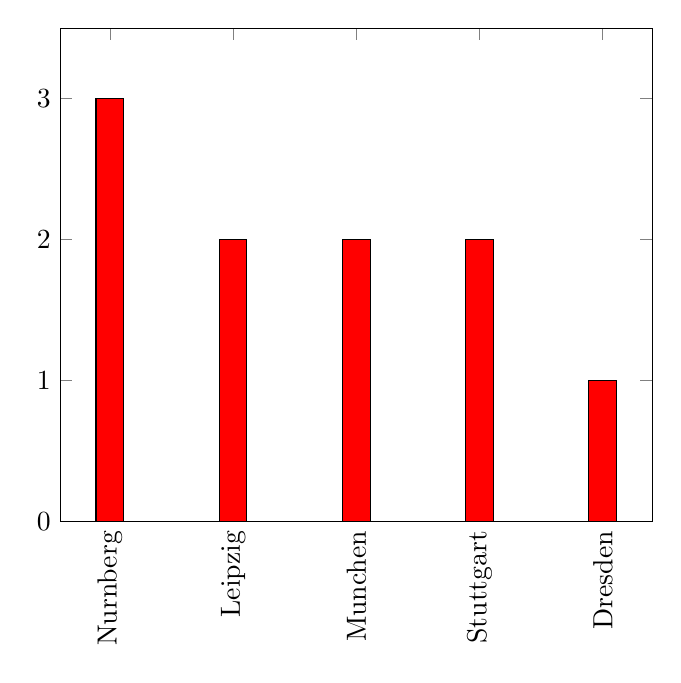
\begin{tikzpicture}
    \begin{axis}[
        width=\textwidth * 0.75,
        symbolic x coords={
            Nurnberg,
            Leipzig,
            Munchen,
            Stuttgart,
            Dresden
        },
        xtick=data,
        x tick label style={rotate=90,anchor=east},
        ymin=0, ymax=3.5, ytick={0,1,2,3}
        ]
        
        \addplot[ybar, fill=red] coordinates {
            (Nurnberg, 3)
            (Leipzig, 2)
            (Munchen, 2)
            (Stuttgart, 2)
            (Dresden, 1)
        };
    \end{axis}
    \end{tikzpicture}
    \caption{Germany Intercity-Express Connected Edges (East South-East Cities)}
    \label{fig:plotjp}
    \end{figure}

%% ref sec
\newpage
\bibliographystyle{ieeetr}
\bibliography{ref.bib}

\end{document}